\documentclass[tikz,border=9pt]{standalone}
\usepackage{lmodern}
\begin{document}
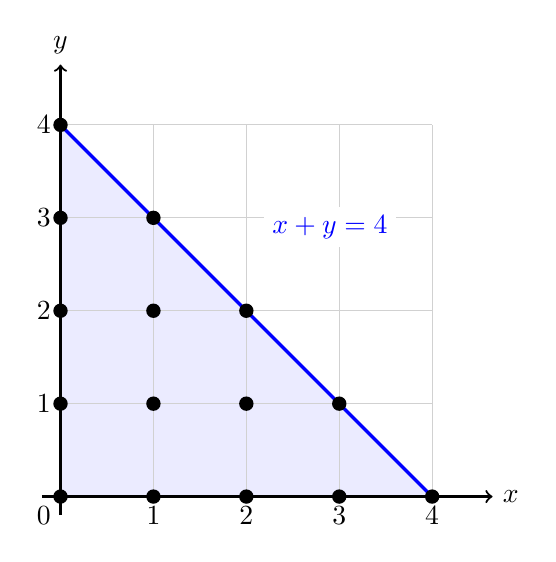
\begin{tikzpicture}[scale=1.18]
  \fill[blue!8] (0,0) -- (4,0) -- (0,4) -- cycle;
  \draw[step=1,black!18] (0,0) grid (4,4);
  \draw[black,thick,->] (-.2,0) -- (4.65,0) node[right] {$x$};
  \draw[black,thick,->] (0,-.2) -- (0,4.65) node[above] {$y$};
  \draw[blue,very thick] (0,4) -- (4,0);
  \foreach \ticknumber in {1,2,3,4} {
    \node[below,black] at (\ticknumber,0) {$\ticknumber$};
    \node[left,black] at (0,\ticknumber) {$\ticknumber$};
  }
  \foreach \a in {0,1,2,3,4} {
    \pgfmathtruncatemacro{\maxb}{4-\a}
    \foreach \b in {0,...,\maxb} {
      \fill[black] (\a,\b) circle[radius=2.2pt];
    }
  }
  \node[below left,black] at (0,0) {$0$};
  \node[blue,fill=white,inner sep=3pt] at (2.9,2.9) {$x+y=4$};
\end{tikzpicture}
\end{document}
